\documentclass[11pt,a4paper]{article}
\usepackage[utf8]{inputenc}
\usepackage[T1]{fontenc}
\usepackage[russian]{babel}
\usepackage[a4paper,
                         left=3cm,
                         top=2cm,
                         right=1.5cm,
                         bottom=2cm,
                         marginparsep=7pt,
                         marginparwidth=.6in]{geometry}
\usepackage{amsmath}
\usepackage{amsfonts}
\usepackage{amssymb}
\usepackage{graphicx}
\usepackage{indentfirst}
\usepackage{pscyr}
\usepackage{hyperref} 
\usepackage{mathtext}
\usepackage{float}
\usepackage{minted}
\usepackage{makecell}
\usepackage{multirow}
\begin{document}
	\thispagestyle{empty}
	\begin{center}
		\textbf{Национальный Исследовательский Университет ИТМО}\\
		\textbf{Факультет Программной Инженерии и Компьютерной Техники}\\
	\end{center}
	\vspace{2em}
	\begin{center}
		
\includegraphics[width=120px]{../../../itmo-logo.png}
	\end{center}
	\LARGE
	\vspace{5em}
	\begin{center}
		\textbf{Вариант № 18}\\
		\textbf{Лабораторная работа № 2}\\
		\Large
		\textbf{по дисциплине}\\
		\LARGE
		\textbf{\emph{'Основы профессиональной деятельности'}}\\
	\end{center}
	\vspace{11em}
	\large
	\begin{flushright}
		\textbf{Выполнил:}\\
		\textbf{Студент группы P3113}\\
		\textbf{\emph{Куперштейн Дмитрий;} : 269359}\\
		\textbf{Преподаватель:}\\
		\textbf{\emph{Перминов Илья Валентинович}}\\
	\end{flushright}
	\vspace{4em}
	\large
	\begin{center}
		\textbf{Санкт-Петербург 2019 г.}
	\end{center}
	\pagebreak{}
	\tableofcontents
	\pagebreak
	\section{Задание}
		По выданному преподавателем варианту определить функцию, вычисляемую программой, область представления и область допустимых значений исходных данных и результата, выполнить трассировку программы, предложить вариант с меньшим числом команд. При выполнении работы представлять результат и все операнды арифметических операций знаковыми числами, а логических операций набором из шестнадцати логических значений.
		\begin{figure}[H]
			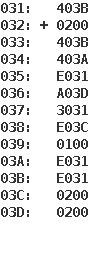
\includegraphics[scale=0.7]{../task.png}
		\end{figure}
	\section{Текст исходной программы с комментариями}
	\begin{table}[H]
		{\tt
	  \begin{tabular}{|c|c|c|c|}
	  	\hline
	  	\textbf{Адрес} & \textbf{Код команды} & \textbf{Мнемоника} &           \textbf{Комментарии}            \\ \hline
	  	     031       &         403B         &       ADD 3B       & Добавить содержимое ячейки памяти 3B к AC \\ \hline
	  	     032       &         0200         &        CLA         &                Очистка AC                 \\ \hline
	  	     033       &         403B         &       ADD 3B       & Добавить содержимое ячейки памяти 3B к AC \\ \hline
	  	     034       &         403A         &       ADD 3A       & Добавить содержимое ячейки памяти 3A к AC \\ \hline
	  	     035 & E031 & ST 31 & Сохранить содержимое AC в ячейку памяти 31\\ \hline
	  	     036 & A03D & LD 3D & Загрузить содержимое ячейки памяти 3D в AC\\ \hline
	  	     037 & 3031 & OR 31 & \makecell{Логически сложить содержимое AC и содержимое\\ ячейки памяти 31 и записать результат в AC}\\ \hline
	  	     038 & E03C & ST 3C & Сохранить содержимое AC в ячейку памяти 3С\\ \hline
	  	     039 & 0100 & HLT & Переход в режим останова\\ \hline
	  	     03A & -- & -- & Данные\\ \hline
	  	     03B & -- & -- & Данные\\ \hline
	  	     03C & -- & -- & Данные\\ \hline
	  	     03D & -- & -- & Данные\\ \hline
	  \end{tabular}
       }
    \end{table}
\section{Описание программы}
\subsection{Назначение и реализуемая функция}
Программа реализует сложение чисел, записанных в ячейках памяти \texttt{3A} и \texttt{3B} и в последсвии производит логическое сложение результата предыдущей операции и набором из 16 логических однобитовых значений, записанное в ячейке памяти \texttt{3D}.

Обозначим число в ячейке памяти \texttt{3A} как $X$, \texttt{3B} как $Y$, набор из 16 однобитовых логических значений ячейки \texttt{3D} как $Z$, а результат (содержимое \texttt{3С}) как $R$:
\begin{equation}
R = (X + Y) \lor Z
\end{equation}
\subsection{ОПИ и ОДЗ}
Область представления:
\begin{itemize}
	\item $R, Z$ -- наборы из 16-ти логических однобитовых значений
	\item $X, Y$ --	 знаковые, 16-ти разрядные числа
\end{itemize}

Область допустимых значений:

Так как $X$ и $Y$ являются знаковыми числами, то для результата их сложения 16-ти битного формата может не хватить, т.е. произойдёт переполнение. Возможно по значению конкретного $X_i$ определить ОДЗ для $Y_i$ по следующей формуле:
\begin{equation}
\begin{cases}
Y_i \in [-2^{15}; \;2^{15} - 1 - X_i], \text{ если } X \geqslant 0\\
Y_i \in [-2^{15} - X_i; 2^{15} - 1], \text{ если } X < 0
\end{cases}
\end{equation}

В качестве упрощения можно определить, что результат будет корректен, когда знаки чисел не совпадают, или когда оба числа равны нулю, или когда бит, предшествующий старшему (знаковому) этих чисел  равен нулю:
\begin{equation}
\left[
\begin{gathered}
\begin{cases}
X \geqslant 0\\
Y\leqslant 0\\
\end{cases}\\
\begin{cases}
X < 0\\
Y> 0\\
\end{cases}\\
-2^{14} \leqslant X, Y \leqslant 2^{14} - 1
\end{gathered}
\right.
\end{equation}

Использование такого упрощения сужает ОДЗ, но позволяет записать его в виде одной системы.
\subsection{Расположение в памяти программы, исходных данных и результата}
\begin{itemize}
	\item Программа: \texttt{031}--\texttt{039}
	\item Исходные данные: \texttt{3A}, \texttt{3B}, \texttt{3D}
	\item Результат: \texttt{3С}
\end{itemize}
\subsection{Адреса первой и последней выполняемой команд программы}
\begin{itemize}
	\item Первая команда: \texttt{031}
	\item Последняя команда: \texttt{039}
\end{itemize}
\pagebreak
\section{Таблица трассировки}
\begin{table}[H]
	\small
	{\tt
	\begin{tabular}{|c|c|c|c|c|c|c|c|c|c|c|c|}
		\hline
		\multicolumn{2}{|c|}{\makecell{\textbf{Выполняемая}\\\textbf{команда}}} & \multicolumn{8}{c|}{\makecell{\textbf{Содержимое регистров процессора после}\\\textbf{выполнения команды.}}} & \multicolumn{2}{c|}{\makecell{\textbf{Ячейка, содержимое}\\\textbf{которой изменилось после}\\\textbf{выполнения команды}}}\\ \hline
		Адрес & Код & IP & CR & AR & DR & SP & BR & AC & NZVC & Адрес & Новый код\\ \hline
		031 & 403B & 032 & 403B & 03B & E031 & 000 & 0031 & E031 & 1000& --& --\\ \hline
		032 & 0200 & 033 & 0200 & 032 & 0200 & 000 & 0032 & 0000 &0100&--&--\\ \hline
	\end{tabular}}
\end{table}
\end{document}